\subsection{``突破瓶颈"}

本项目以实际需求为导向,充分考虑边境安防系统的前述需求,在硬件设备基础上设计软件算法,优化和改善现有方案的不足。
超大场景下的主动目标预测与搜索核心步骤如下:(1)利用边防监控摄像设备,通过调整摄像云台位置(如果定点监控则位置固定不变),焦距、偏转角和俯仰角,得到超大场景内子区域图像,分析并提取图像特征;(2)利用图像特征预测潜在目标相对当前超大场景内子区域的的位置(3)规划路径,通过调整摄像云台使得摄像设备对准目标,完成目标在超大场景内的搜索。
下面从硬件和软件两个方面阐述现有方案的不足与困难。

\textbf{监控摄像设备硬件}行业近年来经历了显著的发展。监控摄像机已经具备了更高的分辨率、动态范围和低光性能。更重要的是,智能化功能如高清图像处理、人脸识别、智能分析等技术的不断发展,使得视频监控系统的功能愈发强大。通过深度学习、计算机视觉等技术的融合应用,视频监控设备具备了更精准的目标识别、行为分析和异常检测能力。

然而,云南边境地区地形复杂,植被覆盖丰富,对监控设备的部署和使用提出了特殊要求。云南省地势西北高、东南低,自北向南呈阶梯状逐级下降,地形地貌复杂多样,包括滇西北的高海拔地区、滇西南的低海拔热带雨林地区等。这些地区植被茂密,地形崎岖,传统的重型监控设备在部署和维护上存在诸多困难。因此,轻量化、便携式的监控设备在云南边境地区具有迫切的需求。轻量化设备不仅便于携带和安装,还能适应复杂的地形和植被环境,提高监控效率和准确性。

针对监控硬件设备,本项目针对云南边境地区的特点,拟采用监控范围广,便携轻量的摄像设备,灵活的开展面向超大场景的边境安防任务,如\reffig{fig:huge-scene-task}(a)所示。

超长变焦能力的监控设备可以在不改变监控位置的情况下,通过调整焦距来捕捉远距离的清晰画面,为超大场景安防监控提供了必要的前提。例如,现有主流便携式长变焦摄像机已实现24-3000 mm等效变焦能力,在能见度较好的天气能够发现10-15千米外的人形目标,如\reffig{fig:huge-scene-task}(b)-(c)所示。
这种超长变焦能力使得监控设备能够在复杂的地形和植被环境中,有效监控远距离的目标,提高监控的效率和准确性。
同时,轻量化和便携式的监控设备也便于集成到无人机或移动机器人上。这种集成方式可以在复杂的遮挡场景中提供更加灵活的监控解决方案。例如,无人机机载摄像设备能够快速调整监控位置、角度和焦距,适应不同的监控需求
,这种灵活性使得监控设备能够在复杂的环境中实现高效监控,提高安防系统的整体性能。
该硬件方案与目前主流的远距离监控摄像设备相比,在成本、体积和重量等方面具有明显优势,更适合云南边境超大场景安防任务,见\reftab{tab:device-comare}。


\begin{figure}[h!]
\centering %图片居中

\includegraphics[width=1\textwidth]{1-2}
\captionsetup{justification=centering} %图题居中
\caption{超大场景边防任务}
\label{fig:huge-scene-task}
\end{figure}


\begin{table}[htbp]
	\zhkai\ensong\selectfont%设置表格字体
	\centering  % 显示位置为中间
	\caption{摄像设备对比}  % 表格标题
	\label{tab:device-comare}  % 用于索引表格的标签
	%字母的个数对应列数,|代表分割线
	% l代表左对齐,c代表居中,r代表右对齐
	\begin{tabular}{l|c|c|c|c|c}  
		\hline  % 表格的横线
		& & & & & \\[-6pt]  %可以避免文字偏上来调整文字与上边界的距离
		设备 & 价格(人民币)&重量&监控范围&安装类型&故障售后 \\  % 表格中的内容,用&分开,\\表示下一行
		\hline
		& &  & & & \\[-6pt]  %可以避免文字偏上 
		远距离监控摄像机 & 47.7 万 (5台起订)& 110 KG & 15KM &地面&研发机构 \\
		便携式长变焦摄像机 & 1.05 万 (量产机)& 1.9 KG & 15KM &地面/机载&全球门店 \\
		\hline
	\end{tabular}
\end{table}

\textbf{现有监控软件及智能化程序}方面,主要围绕以下三个相关领域展开:(1)超大场景下变化物体的图像特征提取(2)超大场景下的动态目标预测(3)面向超大场景的目标主动搜索。然而,在大量文献调查后,申请人发现变化物体有效特征提取、动态环境下的目标主动预测与搜索相关研究较少,同时上述图像特征提取、目标主动预测与搜索 3 个领域的相关技术瓶颈也给本课题带来了困难与挑战。具体分析如下:

(1)\textbf{挑战一:现有图像特征提取方法在超大场景下对变化物体特征提取鲁棒性和泛化能力较差,往往对变化物体和目标识别不完全,给后续潜在目标的预测和搜索带来挑战。}

近年来,基于Transformer的视觉模型\cite{dosovitskiy2020image,carion2020end,liu2021swin,zhu2021deformable,zheng2021rethinking,bao2021beit,he2021masked,liu2021tokens,wang2021pyramid}通过自注意力机制显著提升了图像特征提取的全局建模能力,但其对动态环境下的变化物体(位置和形态等的变化)特征提取能力因分布变化导致鲁棒性和泛化能力大幅下降。同时,对边境安防实时处理和相应的需求,轻量化模型(如DDRNets\cite{DBLP:journals/tits/PanHSJ23})通过降低计算复杂度实现了实时处理,但其在动态环境中的鲁棒性受限于特征表达的局部性。
\reffig{fig:bad-gen-ab}所示为已训练的DDRNets模型\cite{DBLP:journals/tits/PanHSJ23}对新场景的分割效果,DDRNets对新场景下的大部分物体都没有完全识别并分割,只有物体的部分区域分割正确。
\begin{figure}[h!]
\centering %图片居中
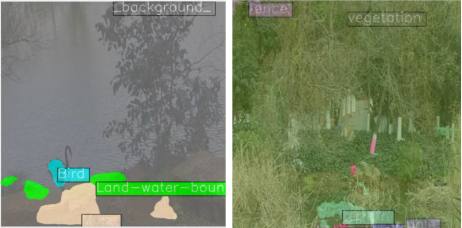
\includegraphics[width=0.8\textwidth]{1-3}
\captionsetup{justification=centering} %图题居中
\caption{已训练的DDRNets模型对新场景的分割效果}
\label{fig:bad-gen-ab}
\end{figure}

图像特征提取的其鲁棒性和泛化能力在目标预测和搜索中至关重要,因为它们能够有效突出关键信息,确保预测和搜索算法在复杂多变的边境环境中稳定运行。
为应对这一问题,现有方法主要通过数据增强,模型优化,迁移学习几种途径实现。
(1)数据增强方面,对原始图像进行数据合成(如随机图像变换\cite{cubuk2020randaugment}、噪声添加\cite{chowdhury2025r}等)或通过学习的方式(如CLUT-Net\cite{mei2022clut})增加数据的多样性和数量,进而提升模型的鲁棒性和泛化能力。
(2)模型优化方面,SGNet \cite{liu2021sg}、CPP-Net \cite{guo2024cpp} 、DynamicCity\cite{dynamiccity2025}、CTA-Net\cite{Meng2024CTA-Net}等新方法通过引入独特的网络结构设计、多尺度特征融合以及注意力机制等,显著提升了图像特征提取模型的泛化能力。
(3)迁移学习方面,CLIP-Adapter\cite{gao2021clip}、TOAST\cite{shi2023toast} 等方法采用轻量级策略,高效地将预训练模型的知识迁移到新的任务或领域中,极大地增强了模型的泛化能力和适应性。
此外,组合式特征提取方法优化也有新进展,CSFF\cite{cheng2020cross}、DilateFormer\cite{jiao2023dilateformer} 等通过多尺度特征提取以及结合传统与深度学习方法,在增强特征的鲁棒性方面具有重要意义。同时,像 FFCA-YOLO \cite{yin2024ffca} 结合了特征增强模块、特征融合模块和空间上下文感知模块,有效增强了小目标的特征表达并抑制复杂背景干扰。这些新方法从不同角度为提升图像特征提取的鲁棒性和泛化能力做出了贡献。

然而,在处理图像损坏、噪声干扰、小样本量以及跨领域任务时,现有方法仍难以充分捕捉因果特征,导致在未见域中的表现欠佳。这些挑战表明,进一步优化特征提取方法以增强模型的泛化能力仍是未来研究的重要方向。\textbf{本项目拟从特征抽象的视角出发,结合图像中物体之间的语义关系与物体局部图像特征,利用图结构表示并充分捕捉变化物体的不变特征,提升模型对复杂多变场景的泛化能力}。

(2)\textbf{挑战二:现有动态图学习方法在超大场景下对稀疏的观测信息利用不够充分,目标潜在位置预测精度和可解释性存在挑战。}


动态图(Dynamic Graph)是指图结构数据在时间维度上发生变化的图。与静态图不同,动态图的
节点、边及其属性可以随时间变化。例如,社交网络中用户之间的关系(边)和用户的信息(节点属
性)会随时间变化;交通网络中道路的流量(边属性)也会随时间变化。动态图通常表示为 ( G =
(A^{(1)}, A^{(2)}, \ldots, A^{(T)}) ),其中 ( A^{(t)} ) 表示第 ( t ) 个时间快照的邻接矩阵,( T ) 是总的时间
步数。动态图的可解释性是指能够清晰地理解、解释动态图模型如何从输入数据中学习到模式、做出预
测或决策的过程。关键方面包括模型的透明性、特征重要性、时间维度的影响、模型决策路径、可视化
与解释工具以及应用领域的特殊需求。
我们的研究任务是计划将摄像头拍摄的一组连续图片转化为动态图,并进行训练,使模型能够预测目
标物体在场景中可能出现的方位。任务的关键步骤包括:
1. 数据预处理:将连续图片转化为动态图,每个节点可以代表图片中的一个物体,边表示物体之间的
关系(如空间距离、运动方向等)。
2. 模型训练:使用动态图神经网络对数据进行训练,学习目标物体在不同时间步的特征和位置信息。
3. 预测与解释:模型训练完成后,能够预测目标物体在新场景中的可能位置,并通过可解释性方法解
释预测结果。
针对研究任务中的以上三个关键步骤,当前已有多种方法能够为我们的研究提供参考:
DyExplainer[1] 是一种专门用于动态图神经网络的可解释性方法,其通过稀疏注意力机制和对比学习技
术,能够实时解释动态图模型的预测结果,同时捕捉结构关系和时间依赖性。具体来说,稀疏注意力机
制通过结构注意力和时间注意力两个模块,捕捉动态图中的关键节点和边,提供更准确的解释。对比学
习技术通过对比学习技术,增强了解释的结构一致性和时间连续性,提高了解释的准确性和可靠性。缓
冲区更新方案通过缓冲区更新方案,建模长期时间依赖性,从而更好地捕捉动态图的时间特性。编码器
无关性使得解释模块是编码器无关的,可以灵活集成到多种动态图神经网络中,适用于大规模动态图网
络。
Causality-Inspired Spatial-Temporal Explanations[2] 则是一种基于结构因果模型的可解释性方
法,旨在通过识别动态图中的琐碎、静态和动态因果关系来解释动态图神经网络的预测。该方法通过以
下技术路线实现:首先,利用对比学习模块区分因果关系和琐碎关系,通过动态相关模块识别动态和静
态因果关系;然后,使用动态变分图自编码器框架生成因果和动态掩码,用于空间和时间解释;最后,
通过对比损失、动态损失、预测损失和稀疏损失等优化生成的掩码,提高解释的准确性和可靠性。该方
法在合成和真实世界数据集上验证了其优越性。
E-SAGE[3] 是一种基于可解释性的防御方法,旨在抵御针对图神经网络的后门攻击。该方法通过评估
图中每条边的重要性,识别出恶意边和良性边之间的显著差异,并通过自适应的迭代修剪过程去除潜在
的恶意边。具体来说,E-SAGE 使用集成梯度方法评估每条边的重要性,生成边缘重要性评分;在预测阶
段,根据边缘评分进行迭代修剪,去除潜在的恶意边;采用邻居采样策略提高计算效率,减少在高维图
数据中的计算负担。通过对比损失、动态损失、预测损失和稀疏损失等优化生成的掩码,提高解释的准
确性和可靠性。该方法在多个数据集和攻击设置下进行了广泛的实验,验证了其有效性和实用性。
T-GAP[4]方法通过引入时间位移编码、多跳推理、注意力传播和子图采样等机制,解决了时序知识图
谱补全中的可解释性问题,能够有效地捕捉时间相关的动态特性,提高模型的预测性能和可解释性。具
体来说,时间位移编码关注每个事件与查询时间戳之间的相对位移,捕捉时间相关的动态;多跳推理通
过逐步扩展节点和边的范围,捕捉复杂的路径信息;注意力传播通过软注意力近似路径遍历,将注意力
值传播到节点的可达邻居节点;子图采样在每个解码步骤中,通过迭代采样查询相关的子图,逐步扩展
节点和边的范围,同时保证关键节点和边的包含。






近年来,相关领域的研究取得了一定进展,例如在轨迹预测方面,有研究提出了基于时空区间信息的Seq2Seq\cite{Seq2SeqTrajRec}框架,用于轨迹恢复,通过结合时空特征和图结构信息,提升了轨迹预测的精度和鲁棒性。还有研究关注即时轨迹预测,如ITPNet\cite{ITPNet},通过集成HiVT\cite{zhou2022hivt}和LaneGCN\cite{liang2020learning}等骨干网络模型,提升了轨迹预测的准确性。然而,这些方法在超大场景下的稀疏观测条件下,仍面临挑战,如特征提取不充分、模型泛化能力不足等,导致目标潜在位置预测精度不高且缺乏可解释性。

如果预测结果缺乏可解释性,那么将使得后续超大场景下的主动搜索过度依赖数据本身,一旦数据中存在噪声和多样环境下的不确定因素,将极大限制设备主动搜索目标的精度。
\textbf{本项目拟使用GNN对动态图结构利用迭代搜索的方式在稀疏的数据样本下获得有效的特征表示,并由此预测目标位置的分布,在此基础上加入GNN可解释机制,得到可信的目标位置预测}。


(3)\textbf{挑战三:现有方法对多条件约束下无法实时处理和规划最优路径,为监控设备主动搜索潜在目标带来挑战。}

主动目标搜索利用之前对潜在目标位置的预测,规划最优路径并控制摄像设备指向目标。
经典路径规划方法在动态多目标场景中面临严重局限,在高频重规划情境下算法的计算开销呈指数级增长\cite{bhardwaj2017learningheuristicsearchimitation}、对密集动态目标时容易产生路径震荡问题\cite{9154607}、或求解时间不可控\cite{10.1145/3272127.3275109},难以满足实时需求。

近年来,数据驱动的方法在路径规划领域取得显著进展(如Neural A\cite{Archetti_2022}, Value Iteration Networks\cite{tamar2017valueiterationnetworks})。基于深度学习和强化学习的路径优化算法也逐渐成为研究热点\cite{zheng2023distributed,cui2024multi,fang2024improved}。
基于深度学习的主动搜索方法\cite{DBLP:conf/iclr/HottungKT22}(Active Search with Deep Learning, ASDL)通过结合强化学习与卷积神经网络(CNN),显著提升了目标搜索的精度与效率。
PriorSparseR-CNN框架\cite{wang2024priorsparse}通过区域生成网络(Region Generation Network, RGN)和特征聚合策略,优化了稀疏目标检测的性能,但其计算复杂度较高,难以满足实时性需求。同时,多目目标爆搜方法(Multi-Objective Explosive Search, MOES)\cite{moes2024}通过生成多个候选目标并结合目标跟踪算法,实现了高精度检测,但其存储空间消耗大,且在处理动态场景时易受目标形变与遮挡影响。
在考虑约束条件的路径规划方面,现有研究能够处理单一或多约束条件下的优化,如自动驾驶场景下在安全性、效率和舒适性之间找到平衡\cite{yang2019generalizedalgorithmmultiobjectivereinforcement}。社会感知运动规划[8](Socially Aware Motion Planning)框架融合深度强化学习技术,使机器人能够理解和预测人类行为,将人的行为作为约束,生成满足条件的导航轨迹,但计算复杂度较高。随后,基于视觉输入的城市导航策略\cite{mirowski2019learningnavigatecitiesmap}实现了无地图导航方法,通过强化学习直接从视觉输入学习导航策略,适用于复杂的城市环境,但对动态环境下的物体处理能力有限。
Think2Drive\cite{li2024think2driveefficientreinforcementlearning}提出了在潜在世界模型中进行"思考"的强化学习框架,通过建立环境的压缩表示,显著减少了对大量物理仿真的依赖,提高了学习效率。

尽管路径优化问题的研究取得了诸多进展,但仍存在以下不足:首先,现有算法在处理大规模动态路径优化问题时,往往面临计算复杂度高、收敛速度慢的问题,难以满足实时性要求。其次,路径优化模型的普适性和灵活性不足,现有方法多针对特定场景设计,难以适应多样化的实际需求。再次,路径优化中的不确定性因素(如交通状况、天气变化)尚未得到充分解决,现有模型的鲁棒性和适应性有待进一步提升。最后,路径优化技术的实际应用仍面临数据安全和隐私保护等挑战,如何在保证数据安全的前提下实现高效优化,仍需进一步研究。
因此,\textbf{本项目拟利用强化学习强大的规划与决策能力,设计适用于多条件约束下的快速训练方法,以支撑边境超大场景下的实时控制和搜索}。
